
\documentclass{beamer}
\usepackage[latin1]{inputenc}
%\usetheme{Montpellier}
%\usetheme{Boadilla}
%\usecolortheme[RGB={204,51,255}]{structure}
%\usecolortheme[named=purple]{structure}
%\usecolortheme[RGB={62,128,62}]{structure}
\usecolortheme[RGB={62,62,128}]{structure}
%\definecolor{reddish}{rgb}{0.3,0.15,0.3}
%\definecolor{light}{rgb}{0.8,0.6,0.8}
%\definecolor{reddish}{rgb}{.5,0.15,0.15}
\definecolor{reddish}{rgb}{0.5,0.3,0.4}
%\definecolor{light}{rgb}{0.8,0.6,0.8}
\definecolor{reddish}{rgb}{.7,0.25,0.25}
\definecolor{greenish}{rgb}{.25,0.8,0.25}
\definecolor{blueish}{rgb}{.25,0.25,0.7}
\definecolor{purple}{rgb}{.5,0.0,0.5}
\usepackage{graphicx}
\usepackage{pstricks}
\usepackage{epsfig}
\newcommand{\btVFill}{\vskip0pt plus 1filll}

\setbeamertemplate{navigation symbols}{}

\newcommand{\crish}{\color{reddish}}
\newcommand{\cgish}{\color{greenish}}
\newcommand{\cbla}{\color{black}}
\newcommand{\cred}{\color{red}}
\newcommand{\cblu}{\color{blue}}
\newcommand{\cgrish}{\color{green}}

\newcommand{\sm}{\color{reddish}$}
\newcommand{\fm}{$\color{black}{}}

\newcommand{\letter}[1]{\color{blue}\texttt{#1}\color{black}}
 \newcommand{\binary}[1]{\color{red}\texttt{#1}\color{black}}

\usepackage{tikz}
\usetikzlibrary{arrows,decorations.markings,positioning}
\usepackage{epstopdf}
\usetikzlibrary{fit}
\usepackage{pgfplots}

\title[The Bayesian Brain lecture 2]{Bayesian fusion: the Bayesian Brain lecture 2}
\author{COMSM0075 Information Processing and Brain}
\institute{\texttt{comsm0075.github.io}}
\date{October 2020}

\begin{document}

\maketitle


\pgfmathdeclarefunction{gauss}{2}{%
  \pgfmathparse{1/(#2*sqrt(2*pi))*exp(-((x-#1)^2)/(2*#2^2))}%
}

\begin{frame}{Bayesian fusion}
  \begin{quote}
    The main topic here is \textbf{Bayesian fusion} but we will introduce it by talking about a nice experiment by Ernst and Banks which demonstrates Bayesian inference in human perception.
  \end{quote}
  \vfill
  \flushright{\tiny{MO Ernst and MS Banks (2002) Humans integrate visual and haptic information in a statistically optimal fashion, 415:429 Nature}}
\end{frame}

\begin{frame}{Ernst and Banks}
\begin{center}
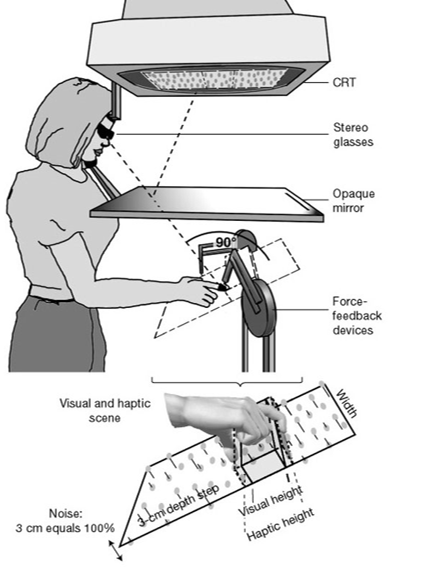
\includegraphics[width=5.5cm]{fig_ernstbanks.png}
\end{center}
  \vfill
  \flushright{\tiny{Pictures from Ernst and Banks}}
\end{frame}


\begin{frame}{Ernst and Banks - vision}
\begin{center}
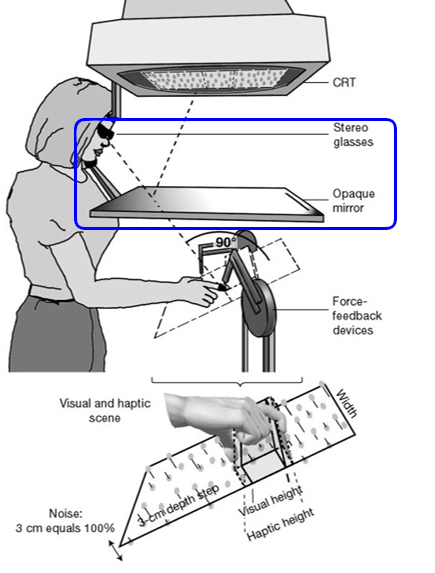
\includegraphics[width=5.5cm]{fig_ernstbanks_vision.png}
\end{center}
  \vfill
  \flushright{\tiny{Pictures from Ernst and Banks}}
\end{frame}


\begin{frame}{Ernst and Banks - touch}
\begin{center}
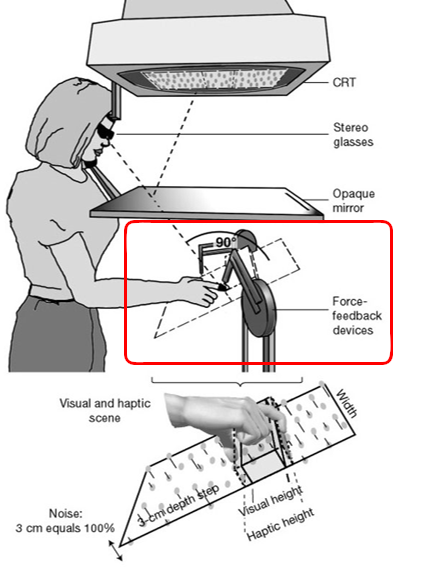
\includegraphics[width=5.5cm]{fig_ernstbanks_haptic.png}
\end{center}
\vfill
  \flushright{\tiny{Pictures from Ernst and Banks}}
\end{frame}

\begin{frame}{Ernst and Banks}
  \begin{itemize}
  \item \crish$x$\cbla{} is the \textbf{true} height of the box.
  \item \cblu$v$\cbla{} is the \cblu\textbf{visual}\cbla{} estimate of the height of the box.
  \item \cred$x$\cbla{} is the \cred\textbf{haptic}\cbla{} estimate of the height of the box.
  \end{itemize}
\vfill
\flushright{\tiny{haptic: of or relating to the sense of touch}}
\end{frame}

\begin{frame}{Estimates are noisy}
\crish$$p(v|x)$$\cbla{} 
  \begin{center}

\includegraphics[width=5.5cm]{box.png}
\end{center}
\end{frame}


\begin{frame}{Estimates are noisy}
\crish$$p(v|x)$$\cbla{} 
  \begin{center}

\includegraphics[width=5.5cm]{blurred_box.png}
\end{center}
\end{frame}

\begin{frame}{Markov chain}
\crish$$
V\rightarrow X\rightarrow H
$$\cbla{}
or
\crish$$
p(v,h|x)=p(v|x)p(h|x)
$$\cbla{}
\end{frame}


\begin{frame}{Markov chain - also called a directed acyclic graph}
\crish$$
V\rightarrow X\rightarrow H
$$\cbla{}
\crish$$
V\leftarrow X\leftarrow H
$$\cbla{}
or
\begin{center}
  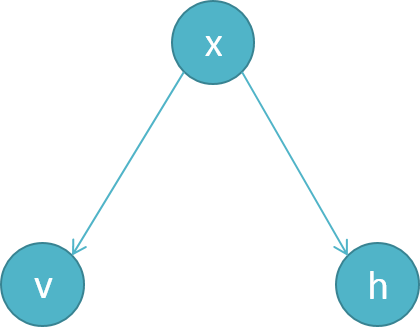
\includegraphics[width=3cm]{fig_dag.png}
\end{center}
\end{frame}


\begin{frame}{Markov chain}

\crish$$
p(v,h|x)=p(v|x)p(h|x)
$$\cbla{}
so
\crish$$
p(v,h,x)=p(v,h|x)p(x)=p(v|x)p(h|x)p(x)
$$\cbla{}
\end{frame}

\begin{frame}{Posterior judgment}
  \crish$$
  p(x|v,h)=\frac{p(v,h|x)p(x)}{p(v,h)}=\frac{p(v|x)p(h|x)p(x)}{p(v,h)}
  $$\cbla{}
\end{frame}

\begin{frame}{MAP estimate}
  Ultimately the participant is asked to estimate the height; we
  assume that they use \crish$p(x|v,h)$\cbla{} and respond with the
  value of \crish$x$\cbla{} which has the maximum value of
  \crish$p(x|v,h)$\cbla{}:
  \crish$$
  \hat{x}=\arg\max_x{p(x|v,h)}
  $$\cbla{}
  This is the \textbf{maximum a posteriori} estimate or \textbf{MAP} estimate.
\end{frame}

\begin{frame}{MAP estimate}
  \crish$$
p(x|v,h)=\frac{p(v,h|x)p(x)}{p(v,h)}=\frac{p(v|x)p(h|x)p(x)}{p(v,h)}
$$\cbla{}
It is assumed that the prior is uniform, so \crish$p(x)$\cbla{} is constant over some range of possible \crish$x$\cbla{}, so if \crish$x$\cbla{} is in that range
\crish$$
p(x|v,h)\propto \frac{p(v|x)p(h|x)}{p(v,h)}
$$\cbla{}
\end{frame}

\begin{frame}{Bayesian fusion}
  Let's assume the noise modelled by \cblu$V$\cbla{} and \cred$H$\cbla{} are Gau\ss{}ian so
\cblu
  \begin{eqnarray*}
    (V|X=x)&\sim{}&\mathcal{N}(x,\sigma_v^2)\cr
    p(v|x)&=&\frac{1}{\sqrt{2\pi\sigma_v^2}}e^{-\frac{(v-x)^2}{2\sigma_v^2}}
  \end{eqnarray*}
  \cbla{}
  and
    \cred
  \begin{eqnarray*}
    (H|X=x)&\sim{}&\mathcal{N}(x,\sigma_h^2)\cr
    p(h|x)&=&\frac{1}{\sqrt{2\pi\sigma_h^2}}e^{-\frac{(h-x)^2}{2\sigma_h^2}}
  \end{eqnarray*}
  \cbla{}
  It is also assumed that the participant has an estimate of the size of the noise, that is, the participant knows \cblu$\sigma_v^2$\cbla{} and \cred$\sigma_h^2$\cbla{}.
\end{frame}
  

\begin{frame}{Bayesian fusion}
So, ignoring any normalization factor
  \crish$$
  p(x|v,h)\propto p(v|x)p(h|x)
  $$\cbla{}
  so we need to multiply the two Gaussians:
  \crish$$
  p(x|v,h)\propto e^{\cblu-\frac{(h-x)^2}{2\sigma_h^2}\cbla}e^{\cblu-\frac{(v-x)^2}{2\sigma_v^2}\cbla}
  $$\cbla{}
  Looking at the exponent we get
\cblu$$
-\frac{(h-x)^2}{2\sigma_h^2}-\frac{(v-x)^2}{2\sigma_v^2}=-\left(\frac{1}{2\sigma_h^2}+\frac{1}{2\sigma_v^2}\right)x^2+\left(\frac{h}{\sigma_h^2}+\frac{v}{\sigma_v^2}\right)x+A
    $$\cbla{}
  where \cblu$A$\cbla{} is other stuff with no \cblu$x$\cbla{}s.
  \end{frame}


\begin{frame}{Bayesian fusion}
\crish$$
-\frac{(h-x)^2}{2\sigma_h^2}-\frac{(v-x)^2}{2\sigma_v^2}=-\left(\frac{1}{2\sigma_h^2}+\frac{1}{2\sigma_v^2}\right)x^2+\left(\frac{h}{\sigma_h^2}+\frac{v}{\sigma_v^2}\right)x+A
    $$\cbla{}
In short
\crish$$
p(x|v,h)\sim \mathcal{N}(\bar{x},\sigma)
$$\cbla{}
where
\crish$$
\frac{1}{\sigma^2}=\frac{1}{\sigma_v^2}+\frac{1}{\sigma_h^2}
$$\cbla{}
and
\crish$$
\bar{x}=\frac{\sigma^2}{\sigma_v^2}v+\frac{\sigma^2}{\sigma_h^2}h
$$\cbla{}
\end{frame}



\begin{frame}{Bayesian fusion}
\crish$$
\frac{1}{\sigma^2}=\frac{1}{\sigma_v^2}+\frac{1}{\sigma_h^2}
$$\cbla{}
Let
\crish$$
\lambda=\frac{\sigma^2}{\sigma_h^2}
$$\cbla{}
then
\crish$$
1-\lambda=\frac{\sigma^2}{\sigma_v^2}
$$\cbla{}
so
\crish$$
\bar{x}=(1-\lambda)v+\lambda h
$$\cbla{}
\end{frame}


\begin{frame}{Bayesian fusion}
  \cblu$v=4$\cbla{} and \cblu$\sigma_v=1$\cbla{}
  \vskip 1cm
\begin{tikzpicture}
  \begin{axis}[
  no markers, domain=0:8, samples=100,
  axis lines*=left, xlabel=$x$, ylabel=$y$,
  every axis y label/.style={at=(current axis.above origin),anchor=south},
  every axis x label/.style={at=(current axis.right of origin),anchor=west},
  height=5cm, width=12cm,
  xtick={4}, ytick=\empty,
  xtick=\empty,
  ytick=\empty,
  enlargelimits=false, clip=false, axis on top,
  grid = major
  ]
  \addplot [very thick,blue] {gauss(4,1)};
\end{axis}
  \draw (7.25,2.2) node{\color{blue}$p(x|v)$\cbla};
\end{tikzpicture}
\end{frame}


\begin{frame}{Bayesian fusion}
  \cred$h=2$\cbla{} and \cred$\sigma_h=1$\cbla{}
  \vskip 1cm
  \begin{tikzpicture}
  \begin{axis}[
  no markers, domain=0:8, samples=100,
  axis lines*=left, xlabel=$x$, ylabel=$y$,
  every axis y label/.style={at=(current axis.above origin),anchor=south},
  every axis x label/.style={at=(current axis.right of origin),anchor=west},
  height=5cm, width=12cm,
  xtick={4}, ytick=\empty,
  xtick=\empty,
  ytick=\empty,
  enlargelimits=false, clip=false, axis on top,
  grid = major
  ]
  \addplot [very thick,red] {gauss(2,1)};
  \end{axis}
    \draw (4.75,2) node{\color{red}$p(x|h)$\cbla};
\end{tikzpicture}
\end{frame}


\begin{frame}{Bayesian fusion}
  \cbla$v=3$\cbla{} and \cbla$\sigma=0.71$\cbla{}
  \vskip 1cm
  \begin{tikzpicture}
  \begin{axis}[
  no markers, domain=0:8, samples=100,
  axis lines*=left, xlabel=$x$, ylabel=$y$,
  every axis y label/.style={at=(current axis.above origin),anchor=south},
  every axis x label/.style={at=(current axis.right of origin),anchor=west},
  height=5cm, width=12cm,
  xtick={4}, ytick=\empty,
  xtick=\empty,
  ytick=\empty,
  enlargelimits=false, clip=false, axis on top,
  grid = major
    ]
    \addplot [very thick,blue] {gauss(4,1)};
    \addplot [very thick,red] {gauss(2,1)};
    \addplot [very thick,black] {gauss(3,0.71)};
\end{axis}
  \draw (5,3.75) node{\color{black}$p(x|v,h)$\cbla};
\end{tikzpicture}
\end{frame}



\begin{frame}{Bayesian fusion}
  \cblu$v=4$\cbla{} and \cblu$\sigma_v=1$\cbla{}
  \vskip 1cm
\begin{tikzpicture}
  \begin{axis}[
  no markers, domain=0:8, samples=100,
  axis lines*=left, xlabel=$x$, ylabel=$y$,
  every axis y label/.style={at=(current axis.above origin),anchor=south},
  every axis x label/.style={at=(current axis.right of origin),anchor=west},
  height=5cm, width=12cm,
  xtick={4}, ytick=\empty,
  xtick=\empty,
  ytick=\empty,
  enlargelimits=false, clip=false, axis on top,
  grid = major
  ]
  \addplot [very thick,blue] {gauss(4,1)};
\end{axis}
  \draw (7.25,2.2) node{\color{blue}$p(x|v)$\cbla};
\end{tikzpicture}
\end{frame}


\begin{frame}{Bayesian fusion}
  \cred$h=2$\cbla{} and \cred$\sigma_h=2$\cbla{}
  \vskip 1cm
  \begin{tikzpicture}
  \begin{axis}[
  no markers, domain=0:8, samples=100,
  axis lines*=left, xlabel=$x$, ylabel=$y$,
  every axis y label/.style={at=(current axis.above origin),anchor=south},
  every axis x label/.style={at=(current axis.right of origin),anchor=west},
  height=5cm, width=12cm,
  xtick={4}, ytick=\empty,
  xtick=\empty,
  ytick=\empty,
  enlargelimits=false, clip=false, axis on top,
  grid = major
  ]
  \addplot [very thick,red] {gauss(2,2)};
  \end{axis}
    \draw (6,2.2) node{\color{red}$p(x|h)$\cbla};
\end{tikzpicture}
\end{frame}


\begin{frame}{Bayesian fusion}
  \cbla$v=3.56$\cbla{} and \cbla$\sigma=0.9$\cbla{}
  \vskip 1cm
  \begin{tikzpicture}
  \begin{axis}[
  no markers, domain=0:8, samples=100,
  axis lines*=left, xlabel=$x$, ylabel=$y$,
  every axis y label/.style={at=(current axis.above origin),anchor=south},
  every axis x label/.style={at=(current axis.right of origin),anchor=west},
  height=5cm, width=12cm,
  xtick={4}, ytick=\empty,
  xtick=\empty,
  ytick=\empty,
  enlargelimits=false, clip=false, axis on top,
  grid = major
    ]
    \addplot [very thick,blue] {gauss(4,1)};
    \addplot [very thick,red] {gauss(2,2)};
    \addplot [very thick,black] {gauss(3.56,0.9)};
\end{axis}
  \draw (5.75,3.5) node{\color{black}$p(x|v,h)$\cbla};
\end{tikzpicture}
\end{frame}

\begin{frame}{Ernst and Banks}
Multiple trials in which the participants are asked to pick which of
two blocks are larger. They use this to estimate the participant's
estimate of the height \crish$\xi$\cbla{} and fit this to
\crish$$
\xi=(1-\mu)v+\mu h
$$\cbla{}
and they then compare \crish$\mu$\cbla{} to \crish$\lambda$\cbla{}:
\crish$$
\bar{x}=(1-\lambda)v+\lambda h
$$\cbla{}
\end{frame}

\begin{frame}{Ernst and Banks}
\begin{center}
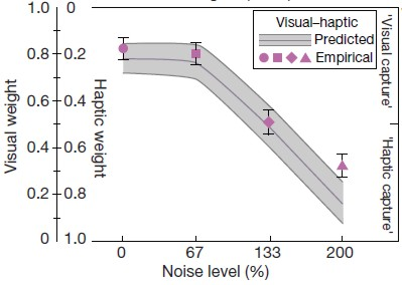
\includegraphics[width=7.5cm]{fig_weights.png}
\end{center}
\vfill
\flushright{\tiny{Figure from Ernst and Banks}}
\end{frame}

\end{document}

